\documentclass{article}

\usepackage{graphicx}
\usepackage{tikz}
\usepackage{tikzsymbols}
\usetikzlibrary{calc,patterns,shapes.geometric}
\pagestyle{empty}
\usepackage[margin=0pt]{geometry}
\geometry{papersize={14in,12in}}

\def\centerarc[#1](#2)(#3:#4:#5){\draw[#1] ($(#2)+({#5*cos(#3)},{#5*sin(#3)})$) arc (#3:#4:#5);}

\begin{document}
	\begin{figure}
		\centering
		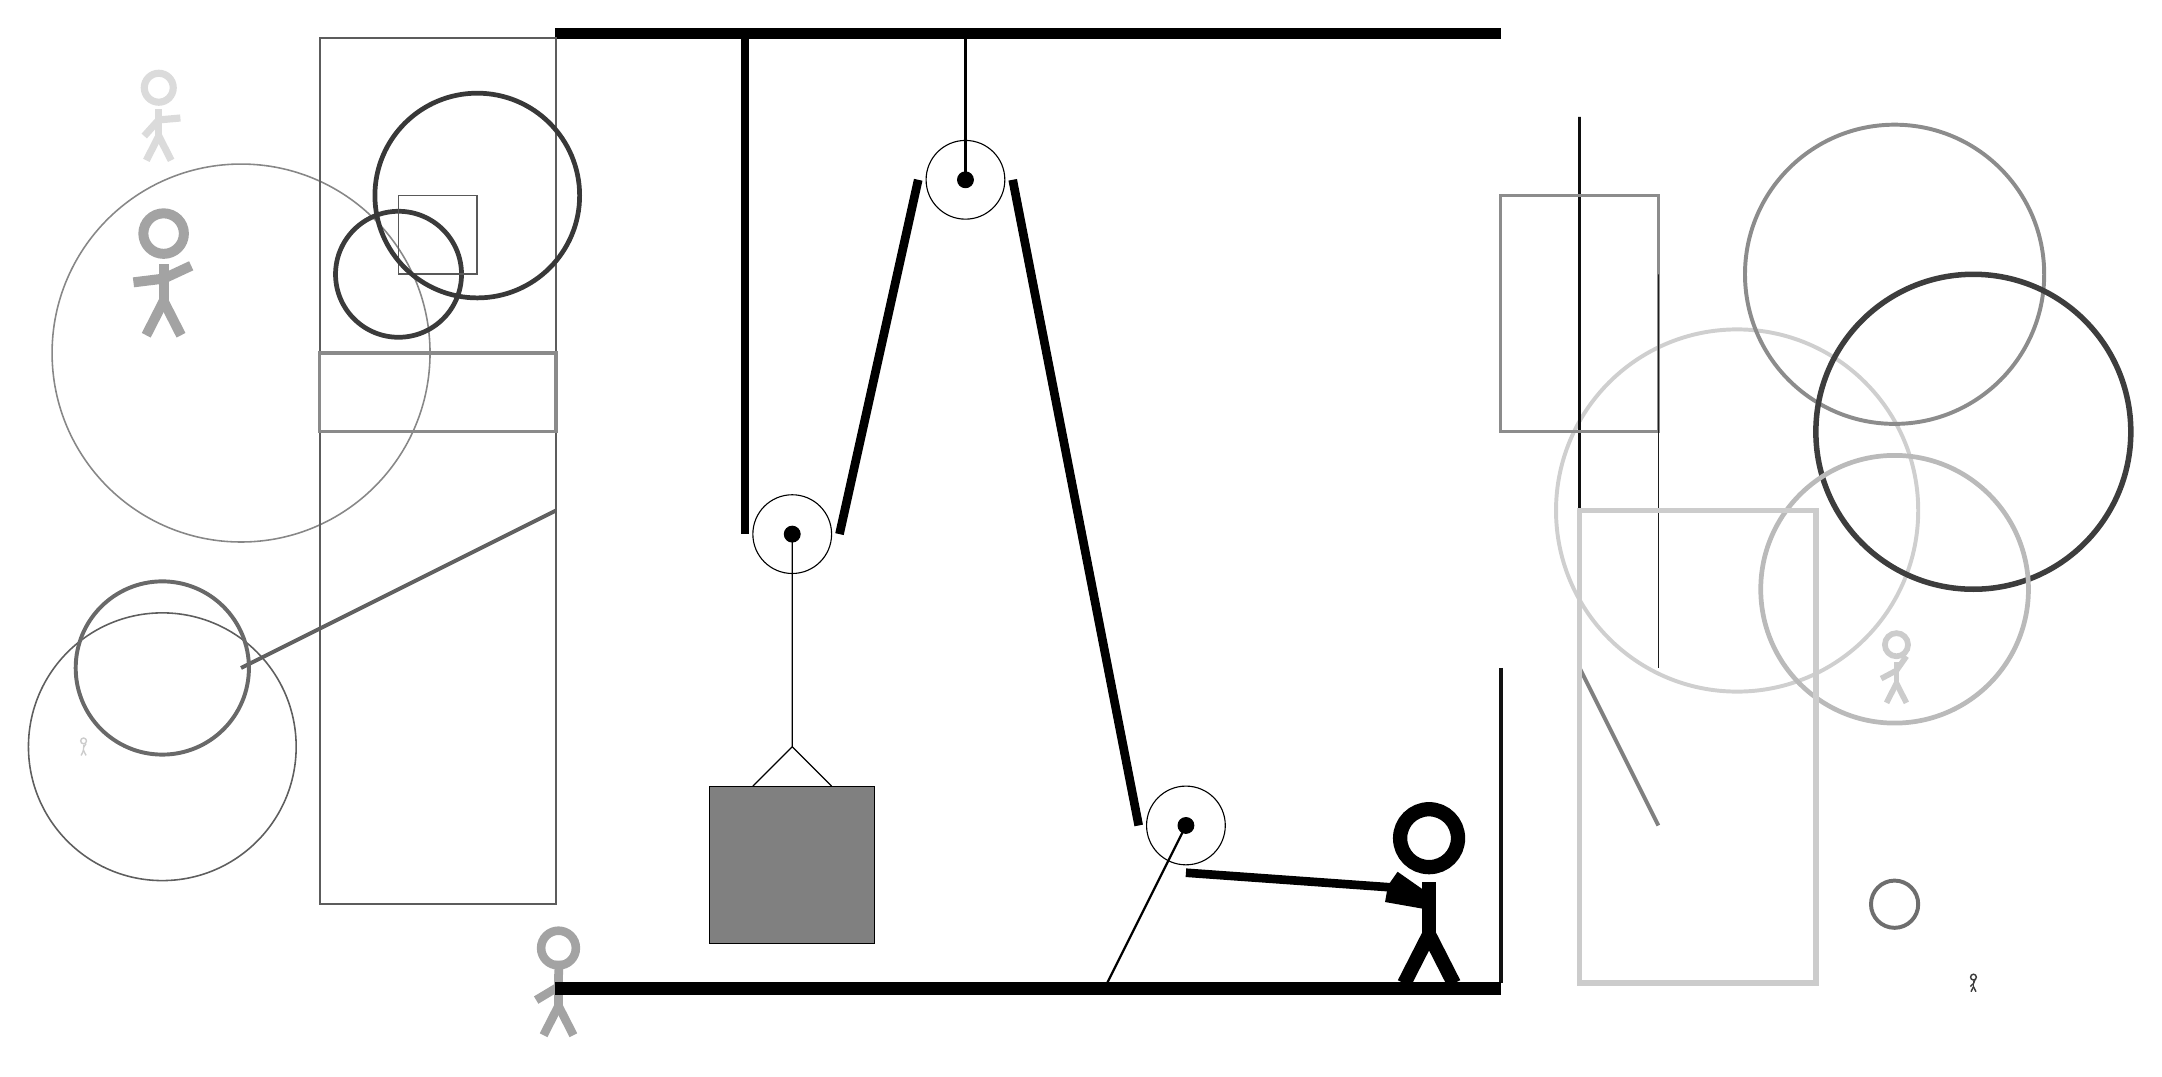
\begin{tikzpicture}
			%%%%% START %%%%%
			
			\draw[fill=black] (-2, 9) rectangle (10, 9.125);
			
			\draw (3.2, 7.2) circle (0.5);
			\draw[fill=black] (3.2, 7.2) circle (0.1);
			\draw[thick] (3.2, 7.2) -- (3.2, 9);
			
			\draw (6, -1) circle (0.5);
			\draw[fill=black] (6, -1) circle (0.1);
			\draw[thick] (6, -1) -- (5, -3);
			
			\draw (1, 2.7) circle (0.5);
			\draw[fill=black] (1, 2.7) circle (0.1);
			
			\draw (1, 2.7) -- (1, 0) -- (0.5, -0.5);
			\draw (1, 0) -- (1.5, -0.5);
			\draw[fill=black!50] (-0.05, -0.5) rectangle (2.05, -2.5);
			
			\draw[line width=1.1mm] (0.4, 9) -- (0.4, 2.7);
			\centerarc[line width=1.1mm](1, 2.7)(180:360:0.6);
			\draw[line width=1.1mm](1.6, 2.7) -- (2.6, 7.2);
			\centerarc[line width=1.1mm](3.2, 7.2)(0:180:0.6);
			\draw[line width=1.1mm](3.8, 7.2) -- (5.4, -1);
			\centerarc[line width=1.1mm](6, -1)(180:270:0.6);
			\draw[line width=1.1mm](6, -1.6) -- (8.8, -1.8);
			
			\node at (9, -1.9) {\Strichmaxerl[10][-35][170]};
			
			\node[line width=0.3mm, color=black!76] at (16, -3) {\Strichmaxerl[1][43][69]};
			
			\draw [line width=0.2mm, color=black!47](-6, 5) circle (2.4);
			\node[line width=0.4mm, color=black!14] at (-7, 8) {\Strichmaxerl[5][48][5]};
			\draw [line width=0.5mm, color=black!19](13, 3) circle (2.3);
			
			\draw [line width=0.5mm, color=black!45](15, 6) circle (1.9);
			
			\draw[line width=0.5mm, color=black!50](11, 1) -- (12, -1);
			\draw[line width=0.3mm, color=black!94] (11, 8) rectangle (11, 0);
			
			\draw[line width=0.5mm, color=black!62](-2, 3) -- (-6, 1);
			\draw[line width=0.4mm, color=black!45] (10, 7) rectangle (12, 4);
			\draw[line width=0.2mm, color=black!89] (12, 6) rectangle (12, 1);
			\draw[line width=0.5mm, color=black!45](14, -3) -- (12, -3);
			\node[line width=0.2mm, color=black!36] at (-7, 6) {\Strichmaxerl[7][7][25]};
			\draw [line width=0.7mm, color=black!76](16, 4) circle (2.0);
			
			\draw [line width=0.2mm, color=black!63](-7, 0) circle (1.7);
			\draw[line width=0.2mm, color=black!64] (-2, 9) rectangle (-5, -2);
			\draw[line width=0.4mm, color=black!46] (-2, 4) rectangle (-5, 5);
			\draw [line width=0.5mm, color=black!59](-7, 1) circle (1.1);
			\node[line width=0.5mm, color=black!20] at (-8, 0) {\Strichmaxerl[1][87][57]};
			\draw [line width=0.6mm, color=black!77](-4, 6) circle (0.8);
			\draw[line width=0.5mm, color=black!93](10, 1) -- (10, -3);
			\draw [line width=0.5mm, color=black!57](15, -2) circle (0.3);
			
			\draw[line width=0.2mm, color=black!65] (-3, 6) rectangle (-4, 7);
			\node[line width=0.6mm, color=black!20] at (15, 1) {\Strichmaxerl[4][28][55]};
			\node[line width=0.4mm, color=black!36] at (-2, -3) {\Strichmaxerl[6][31][89]};
			\draw [line width=0.6mm, color=black!27](15, 2) circle (1.7);
			
			\draw[line width=0.7mm, color=black!20] (11, -3) rectangle (14, 3);
			\draw [line width=0.6mm, color=black!78](-3, 7) circle (1.3);
			
			\draw[fill=black] (-2, -3) rectangle (10, -3.15);
			
			%%%%% END %%%%%
		\end{tikzpicture}
	\end{figure}	
\end{document}